The filter design process is documented in this section, which includes determination of filter specifications, implementation and test. As stated in section \ref{sec:filtervalg} a bandpass FIR filter of type 1 designed with use of a Kaiser window is desired.

\subsection{Specifications of filter} \label{sec:FIRspec} 
The purpose of this filter is to remove all frequencies outside the passband of the filter. As stated in section \ref{sec:filtervalg} the frequencies the analysed signals are located within a frequency band from 82 Hz to 1000 Hz.  
By letting the cut-off frequencies of the filter be $f_{c1}=70$ Hz and $f_{c2}=1000$ Hz, respectively, this specifies the passband of the filter. \\
According to section \ref{subsec:FIR} the Kaiser window can be determined from specifications of the allowed transition width $tw$, which is similar to $\Delta \omega$ specified in Hz, and peak approximation error $\delta$ of the amplitude in the pass- and stopbands. \\ 
By the frequency analysis of different types of noise it is found that the frequency spectrum of the music signal lies within the frequency spectrum of the noise, which verifies the need of a narrow transitionband. However, a narrow transitionband means that a higher order of filter is needed, which gives more computations, and hence it is not realistic to let the width of the transitionband go towards zero.  \\
The maximum allowed width of the transitionband $tw$ and peak approximation error in amplitude $\delta$ is determined as
\begin{align}
tw = 20 \ \text{Hz}, \ \ \ \ \  \delta = 0.05. 
\end{align}
The amplitude response of the ideal filter is sketched in figure \ref{fig:spec_Hd} along with the boundaries for the realisable filter as provided by the defined specifications.      
\begin{figure}[H]
\centering
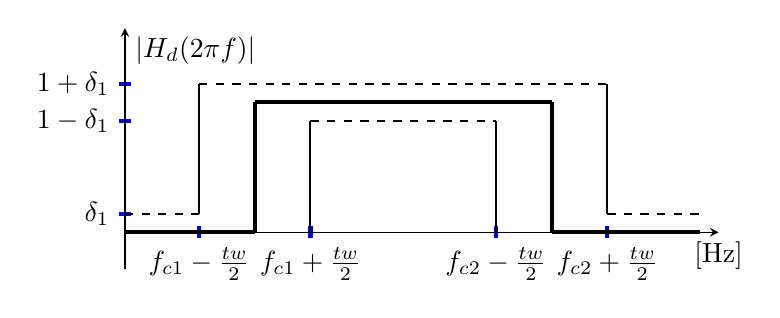
\begin{tikzpicture}[scale=1]
\begin{axis}[every tick/.style={blue, ultra thick}, 
scale=1.1,
unit vector ratio*=1 1 1,
axis lines = middle,
x label style={at={(current axis.right of origin)},anchor=north},
xlabel={[Hz]},
xtick={2,5,10,13},
xticklabels={$f_{c1}-\frac{tw}{2}$,$f_{c1}+\frac{tw}{2}$,$f_{c2}-\frac{tw}{2}$,$f_{c2}+\frac{tw}{2}$},
ytick={0.5,3,4},
yticklabels={$\delta_1$,$1-\delta_1$,$1+\delta_1$},
xmin=0,
xmax=16,
ymin=-1,
ymax=5.5]
\node at (axis cs:1.9,4.9) {$|H_d(2\pi f)|$};
\draw[line width=0.5mm](axis cs:0,0)--(axis cs:3.5,0);
\draw[line width=0.5mm](axis cs:3.5,0)--(axis cs:3.5,3.5);
\draw[line width=0.5mm](axis cs:3.5,3.5)--(axis cs:11.5,3.5);
\draw[line width=0.5mm](axis cs:11.5,3.5)--(axis cs:11.5,0);
\draw[line width=0.5mm](axis cs:11.5,0)--(axis cs:15.5,0);
\draw[line width=0.25mm, dashed](axis cs:0,0.5)--(axis cs:2,0.5);
\draw[line width=0.25mm, dashed](axis cs:13,0.5)--(axis cs:15.5,0.5);
\draw[line width=0.25mm, dashed](axis cs:5,3)--(axis cs:10,3);
\draw[line width=0.25mm, dashed](axis cs:2,4)--(axis cs:13,4);
\draw[line width=0.25mm](axis cs:2,0.5)--(axis cs:2,4);
\draw[line width=0.25mm](axis cs:5,0)--(axis cs:5,3);
\draw[line width=0.25mm](axis cs:10,0)--(axis cs:10,3);
\draw[line width=0.25mm](axis cs:13,4)--(axis cs:13,0.5);
%\draw[line width=0.5mm](axis cs:4,0.5)--(axis cs:7,0.5);
%\node at (axis cs:1,1.5) {Passband};
%\node at (axis cs:3,1.5) {Transition};
%\node at (axis cs:5.0,1.5) {Stopband};
\end{axis}
\end{tikzpicture}
\caption{Amplitude response of ideal filter within the boundaries for the amplitude response of the realisable filter as given by the defined specifications.}
\label{fig:spec_Hd}
\end{figure}

\subsection{Implementation of filter}
The implementation of the filter basically follows algorithm \ref{alg:FIR}. The ideal impulse response is defined as the inverse Fourier transform of the ideal filter specified in figure \ref{fig:spec_Hd}. The derivation of the ideal impulse response of a bandpass filter is shown in appendix \ref{appC}. From the given specifications the shape parameter of the Kaiser window becomes $\beta \approx 1.5$, which gives a filter order of $M=2766$. Figure \ref{fig:FIRimpulse} shows the impulse response of the filter. Figure \ref{fig:freq_filt1} illustrates a plot of the amplitude response corresponding to the filter in the frequency domain. Figure \ref{fig:freq_filt2} illustrates a close-up view of the left transitionband, showing the ripples in the stop- and passband. The boundaries from the specifications are marked by the green lines. It is seen that the specifications are fulfilled to a certain degree. 
\begin{figure}[h]
\centering 
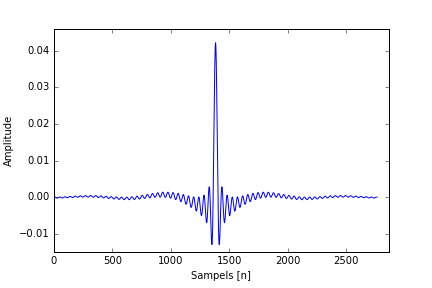
\includegraphics[scale=0.5]{figures/filtertest/impulse.png}
\caption{Impulse response of filter with order $M=2766$.}
\label{fig:FIRimpulse}
\end{figure}
       
\begin{figure}[h]
\centering
\begin{subfigure}{0.49\textwidth}
\centering
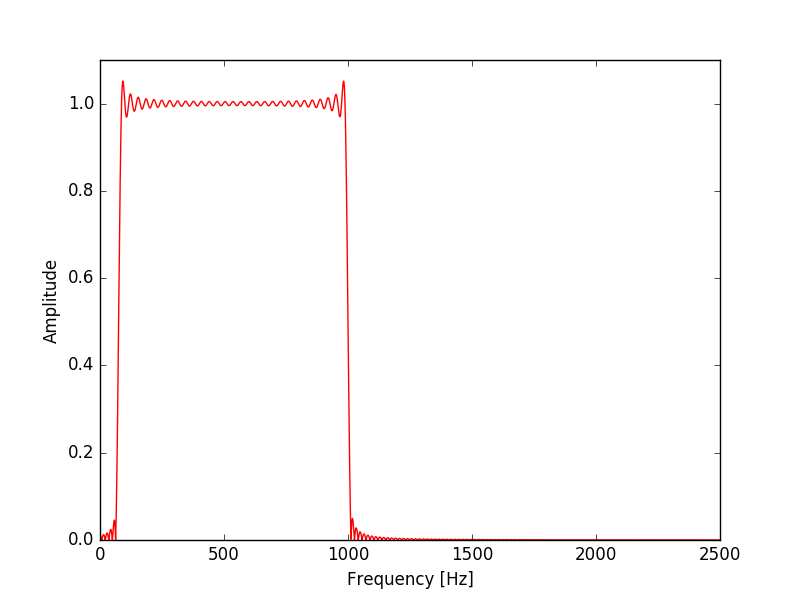
\includegraphics[width=\textwidth]{figures/filtertest/freq_response1.png}
\caption{}
\label{fig:freq_filt1}
\end{subfigure}
\begin{subfigure}{0.49\textwidth}
\centering
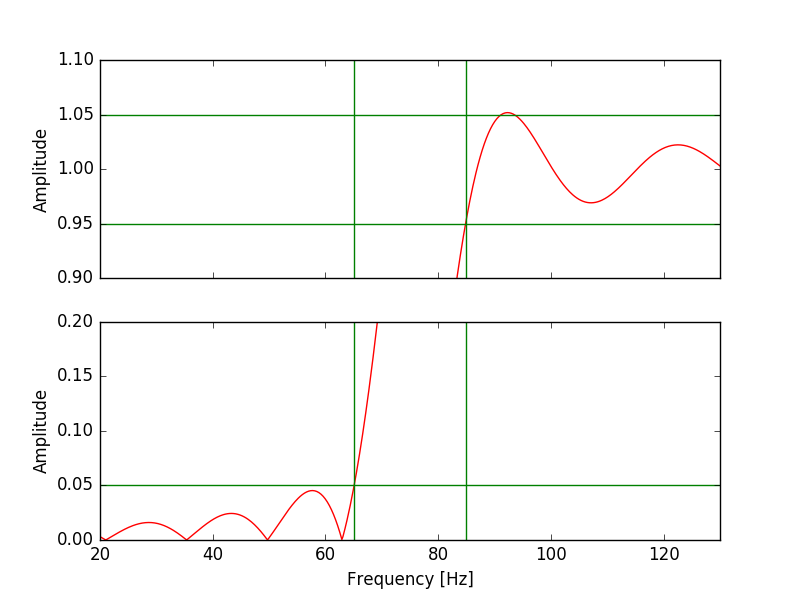
\includegraphics[width=\textwidth]{figures/filtertest/freq_response2.png}
\caption{}
\label{fig:freq_filt2}
\end{subfigure}
\caption{\textbf{(a)} Amplitude response of filter. \textbf{(b)} Close-up view of amplitude response of filter, showing top and bottom of one transitionband.}
\label{fig:freq_filt}
\end{figure}

\begin{algorithm}
\caption{Compute type 1 FIR filter}
\label{alg:FIR}
\begin{algorithmic}[1] 
\Procedure{Compute kaiser window}{$\delta,f_s,tw$}
\State $A=-20\log_{10}(\delta)$ \Comment{$21 \leq A \leq 50$}
\State $\beta = 0.5824(A-21)^{0.4} + 0.07886(A-21)$ \Comment {Shape parameter}
\State $M = (A-8)/(2.285 \cdot \frac{tw}{f_s} 2\pi)$ \Comment {Filter order, rounded up to even int.}
\State $N = M+1$ \Comment {Length of filter}
	\For {each $i$ in length of $N$}
		\For {each $j$ in length of $M$}
			\State $ sum_n$ += $ \ (\frac{1}{j!})^2 \left( \left( \frac{\beta}{2} \sqrt{\left(1 - \left( \frac{2 \cdot i}{N-1}\right) - 1\right)^2}\right)^{2j}\right)$
			\State $ sum_d$ += $\ (\frac{1}{j!})^2 \left( \frac{\beta}{2}\right)^{2j}$
		\EndFor
		\State $w[i]=\frac{sum_n}{sum_d}$
	\EndFor
	\State Return $w$, $M$, $N$
\EndProcedure
\\
\Procedure{Compute ideal impulse response}{$M,f_{c1},f_{c2},f_s,N$}
   \For {each $i$ in length of $N$}
        \If {$i == \frac{M}{2}$}
        		\State $h_d[i] = 2( \frac{f_{c2}}{f_s} - \frac{f_{c1}}{f_s})$
        	\Else 
        		\State  $h_d[i] = \frac{1}{ (\pi (i - \frac{M}{2}))}(\sin(\frac{f_{c2}}{f_s} 2 \pi (i - \frac{M}{2})) - (\sin(\frac{f_{c1}}{f_s} 2 \pi (i - \frac{M}{2}))))$ 
          	\EndIf 
  	\EndFor
  	\State Return $h_d$
\EndProcedure
\\
\Procedure{Compute impulse response}{$h_d,w$}
	\State Return $h = h_d \cdot w$ \Comment{Windowed impulse response}
\EndProcedure
\end{algorithmic}
\end{algorithm}

\subsection{Test of filter}
The implemented filter is tested according to the test specifications described in section \ref{sec:testspec}. Figure \ref{fig:SIGNAL} shows the frequency spectrum of the single $E_2$ tone with additive noise in form of a beat of hands clapping. Figure \ref{fig:filt_SIGNAL} shows the filtered signal obtained by multiplying the signal with the filter in frequency domain. Note that the frequency spectra are only showed from 0 to approximately 2200 Hz.  

\begin{figure}[H]
\centering
\begin{subfigure}{0.49\textwidth}
\centering
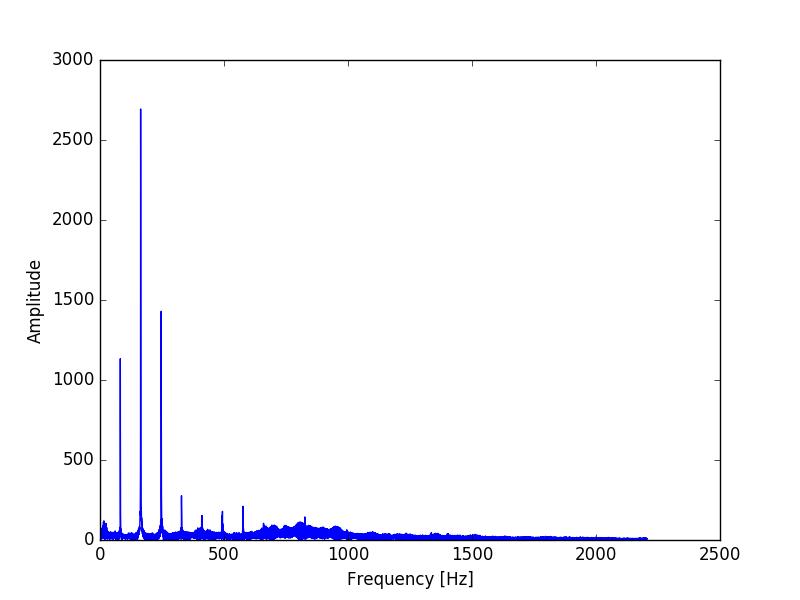
\includegraphics[width=\textwidth]{figures/filtertest/SIGNAL.png}
\caption{}
\label{fig:SIGNAL}
\end{subfigure}
\begin{subfigure}{0.49\textwidth}
\centering
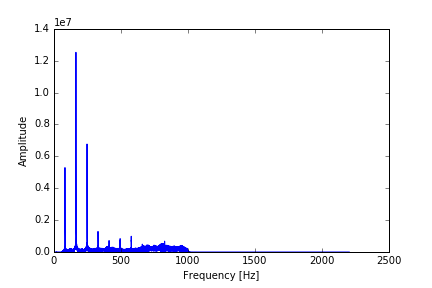
\includegraphics[width=\textwidth]{figures/filtertest/f_SIGNAL.png}
\caption{}
\label{fig:filt_SIGNAL}
\end{subfigure}
\caption{\textbf{(a)} Frequency spectrum of signal with noise. \textbf{(b)} Frequency spectrum of filtered signal.}
\label{fig:test_res}
\end{figure}
As described in the specifications the filter is designed to remove all frequencies outside the frequencyband from 70 Hz to 1000 Hz. It is seen by comparing figure \ref{fig:SIGNAL} and figure \ref{fig:filt_SIGNAL} that the frequencies outside the passband appears to be zero and that the amplitudes of the remaining frequencies are approximately the same. \\
The designed filter of order 2766 is seen to fulfil the specifications, and the implementation of the filter is shown to work as intended. \\